\section{Training Process}

The training process begins with the initialization of the ResNet-34
backbone using pre-trained weights, providing a strong foundation for
feature extraction. The model's hyperparameters are optimized using
Optuna \cite{AkibaEtAl2019}, a hyperparameter optimization framework
that employs Bayesian
optimization to search for optimal values of:

\begin{itemize}
  \item Learning rate: Sampled logarithmically between $10^{-5}$
    and $10^{-2}$
  \item TGCE$_{SS}$ parameters:
    \begin{itemize}
      \item $q$: Controls truncation of the loss function (0.1 to 0.9)
      \item Noise tolerance: Controls model's robustness to label
        noise (0.1 to 0.9)
      \item Regularization weights: Control the balance between
        different loss terms.
    \end{itemize}
\end{itemize}

Two separate hyperparameter optimization studies were conducted using Optuna,
each with 20 iterations, on the Oxford PET dataset with three scorers
emulating SNR noises of -20, 0, and 10 dB respectively, and a labeling
rate of 0.5. The first study focused exclusively on regularization
parameters with preselected values of $q=0.66$, $\tilde{C}=0.62$, and
learning rate $=6.5 \times 10^{-4}$, aiming to determine the relative
importance of different regularizers. The second study was comprehensive,
including the mandatory loss function parameters ($q$, $\tilde{C}$) and
learning rate, which are more sensitive to changes and directly affect
the loss function and optimizer behavior.

Table~\ref{tab:hyperparameter_importance_regularizers} presents the
hyperparameter importance ranking for the regularizers-only study, while
Table~\ref{tab:hyperparameter_importance_comprehensive} shows the
results from the comprehensive study including all parameters.

\begin{table}[h]
  \centering
  \begin{tabular}{lc}
    \toprule
    \textbf{Hyperparameter} & \textbf{Importance Score} \\
    \midrule
    $\beta_\lambda$ & 0.4728 \\
    $\alpha_{\text{sum}}$ & 0.1364 \\
    $\alpha_{\text{entropy}}$ & 0.1291 \\
    $\alpha_{\lambda}$ & 0.1280 \\
    $\alpha_{\text{centroid}}$ & 0.0997 \\
    $\gamma_\lambda$ & 0.0340 \\
    \bottomrule
  \end{tabular}
  \caption{Hyperparameter importance ranking for regularization parameters
    obtained from Optuna optimization study after 20 iterations. This study
    used preselected values of $q=0.66$, $\tilde{C}=0.62$, and learning
    rate $=6.5 \times 10^{-4}$. The importance scores indicate the relative
  impact of each regularization hyperparameter on the model's performance.}
  \label{tab:hyperparameter_importance_regularizers}
\end{table}

\begin{table}[h]
  \centering
  \begin{tabular}{lc}
    \toprule
    \textbf{Hyperparameter} & \textbf{Importance Score} \\
    \midrule
    $\text{learning\_rate}$ & 0.2267 \\
    $q$ & 0.1832 \\
    $\tilde C$ & 0.1480 \\
    $\alpha_{\lambda}$ & 0.1127 \\
    $\alpha_{\text{sum}}$ & 0.0988 \\
    $\alpha_{\text{entropy}}$ & 0.0868 \\
    $\alpha_{\text{centroid}}$ & 0.0380 \\
    $\beta_\lambda$ & 0.0821 \\
    $\gamma_\lambda$ & 0.0237 \\
    \bottomrule
  \end{tabular}
  \caption{Comprehensive hyperparameter importance ranking including all
    parameters obtained from Optuna optimization study after 20 iterations.
    This study shows the relative importance of mandatory loss function
    parameters ($q$, $\tilde{C}$), learning rate, and regularization
  parameters together.}
  \label{tab:hyperparameter_importance_comprehensive}
\end{table}

After finding the optimal hyperparameters, the model is trained end-to-end
using the Adam optimizer with the best learning rate found
\footnote{For every experiment this was also tuned with the help of
the Optuna study, having different optimal values for every experiment.}. The
TGCE$_{SS}$ loss function plays a crucial role in updating both the
segmentation and reliability branches, ensuring that the model learns
to effectively handle multiple annotators' inputs while accounting
for their varying reliability.

\begin{figure}[h]
  \centering
  \begin{tikzpicture}[
      node distance=1.2cm and 1.5cm,
      every node/.style={font=\footnotesize},
      box/.style={draw, rectangle, minimum width=2.5cm, minimum
      height=1cm, align=center},
      arrow/.style={-{Latex}, thick},
      roundedbox/.style={draw, rectangle, rounded corners=5pt,
      minimum width=4.2cm, minimum height=1.2cm, align=center}
    ]

    % Dataset notation
    \node[align=left] (dataset) at (-4.5,1.5) {
      \textbf{Train Dataset} \\
      $\left\{(x_n, \tilde{y}^r_n)\right\}_{r \in R_n}^{n \in \mathbb{N}}$
    };

    % Image box
    \node[box, right=2cm of dataset] (image) {%
      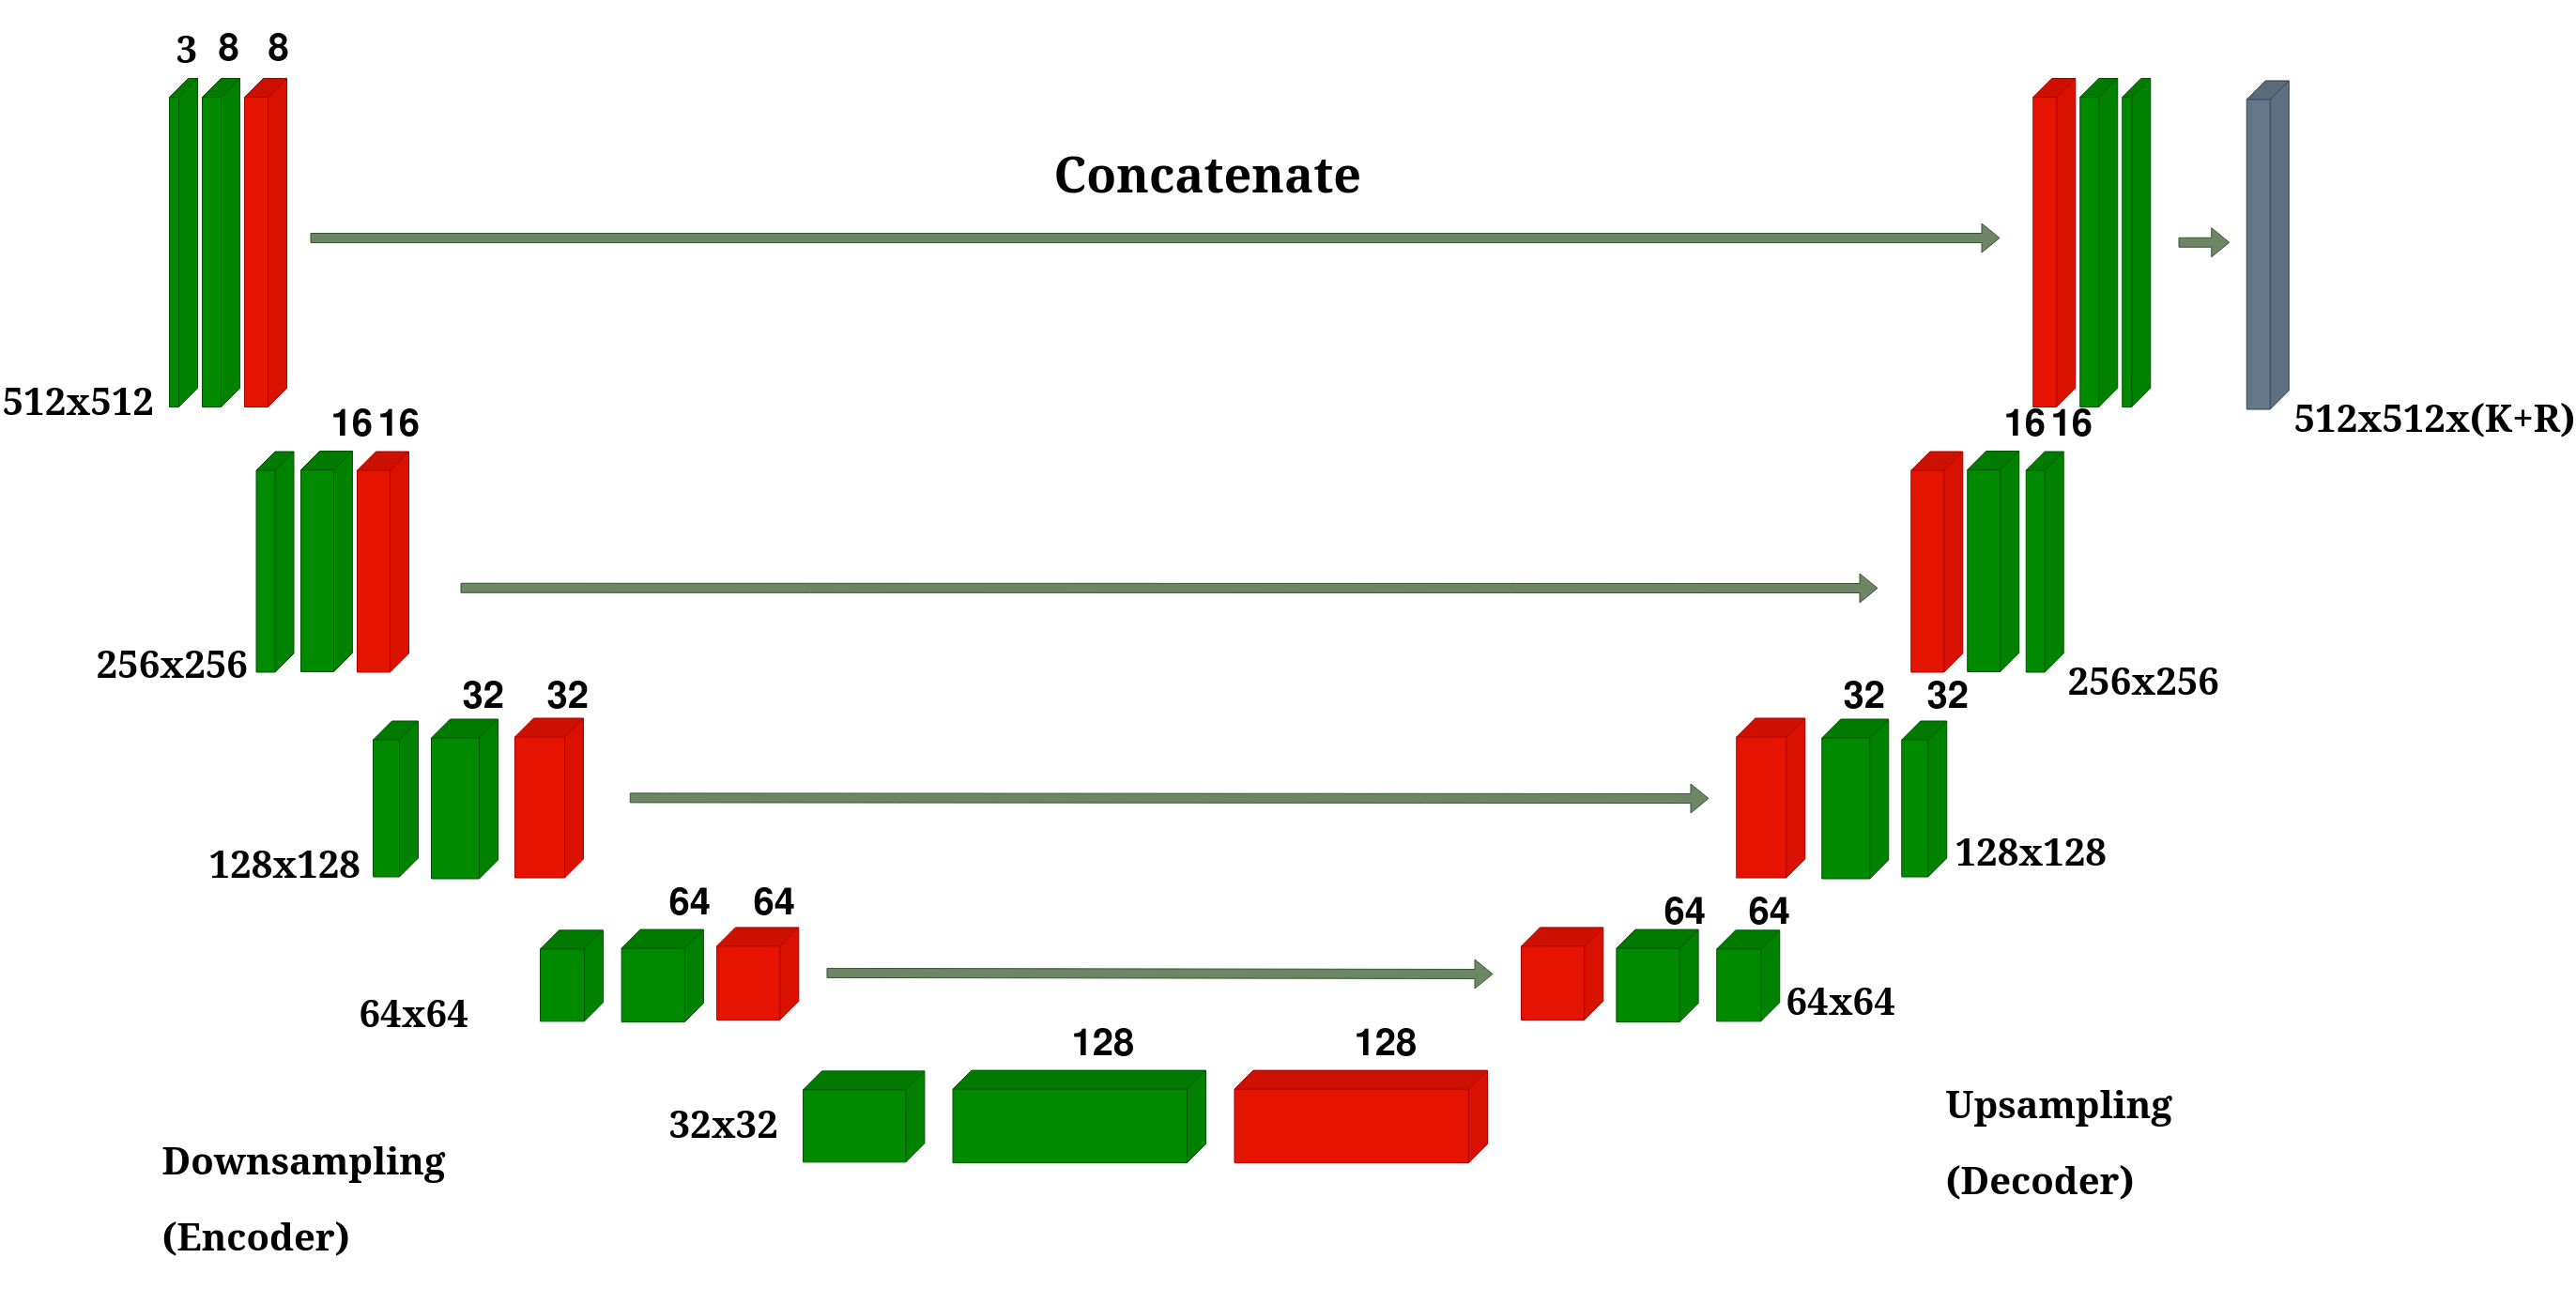
\includegraphics[width=2.5cm]{Cap5/Figures/cnn_arch_overview.png}
    };

    % Output of model
    \node[align=left, right=of image] (modelout) {
      $\left[ f(x; \theta), \; \Lambda_r(x; \theta) \right]$
    };

    % Loss function / objective set
    \node[roundedbox, below=0.7cm of modelout] (loss) {%
      $TGCE_{\text{SS}}(Y_r, f(x;
      \theta) \mid r, \Lambda_r(x; \theta))$
    };

    % Argmin
    \node[box, below=of loss] (argmin) {
      $\argmin_{\theta} \mathcal{L}(\theta)$
    };

    % Hyperparameter tuning
    \node[roundedbox, below=0.7cm of argmin] (tuner) {%
      Bayesian Optimization \\
      $\argmax_{\phi} \text{Dice}(f(x; \theta))$
    };

    % Arrows
    \draw[arrow] (dataset) -- (image);
    \draw[arrow] (image) -- (modelout);
    \draw[arrow] (modelout) -- (loss);
    \draw[arrow] (dataset) |- (loss);
    \draw[arrow] (loss) -- (argmin);
    \draw[arrow] (argmin) -- (tuner);

  \end{tikzpicture}
  \caption{Training process of the proposed model overview. The model first
    undergoes hyperparameter optimization using Bayesian optimization,
    followed by end-to-end training with the optimal parameters.
    Estimated segmentation and reliability maps are computed for each input
    image, and the loss function is computed for the entire batch.
    Network parameters are tuned based on the loss function as
    objective (with minimization target) whereas the hyperparameters
    $\phi$ tuning are based on the Dice coefficient of the validation
  data set (with maximization target). }
  \label{fig:optimization_process}
\end{figure}

The model's architecture is specifically designed to address the
challenges of multi-annotator segmentation. Through the ResNet-34
backbone, it learns robust segmentation features that capture
high-level patterns in the data. The UNET's skip connections enable
the preservation of fine-grained details, while the parallel
reliability branch allows the model to adapt to annotator-specific
characteristics. This comprehensive design enables the model to
effectively handle multiple annotators' inputs while maintaining high
segmentation accuracy and reliability estimation.
